\section{北京理工大学本科生毕业设计论文模板使用指南} \label{grad-thesis}

\tipbox{注意:目前版本的毕业设计论文已经按照北京理工大学 2016 级(2020 届)毕业论文模板进行的设计与排版的更新。}

本模板已经发布在 Overleaf 上,你可以打开直接使用(点击下图 \ref{overleaf-grad-thesis} 所示中的 Open as Template 即可:

\begin{center}
  \color{ForestGreen}\href{https://www.overleaf.com/latex/templates/bei-jing-li-gong-da-xue-ben-ke-sheng-bi-ye-she-ji-lun-wen-mo-ban/mwhjgqsncxxg}{https://www.overleaf.com/latex/templates/bei-jing-li-gong-da-xue-ben-ke-sheng-bi-ye-she-ji-lun-wen-mo-ban/mwhjgqsncxxg}
\end{center}

\begin{figure}[H]
  \centering
  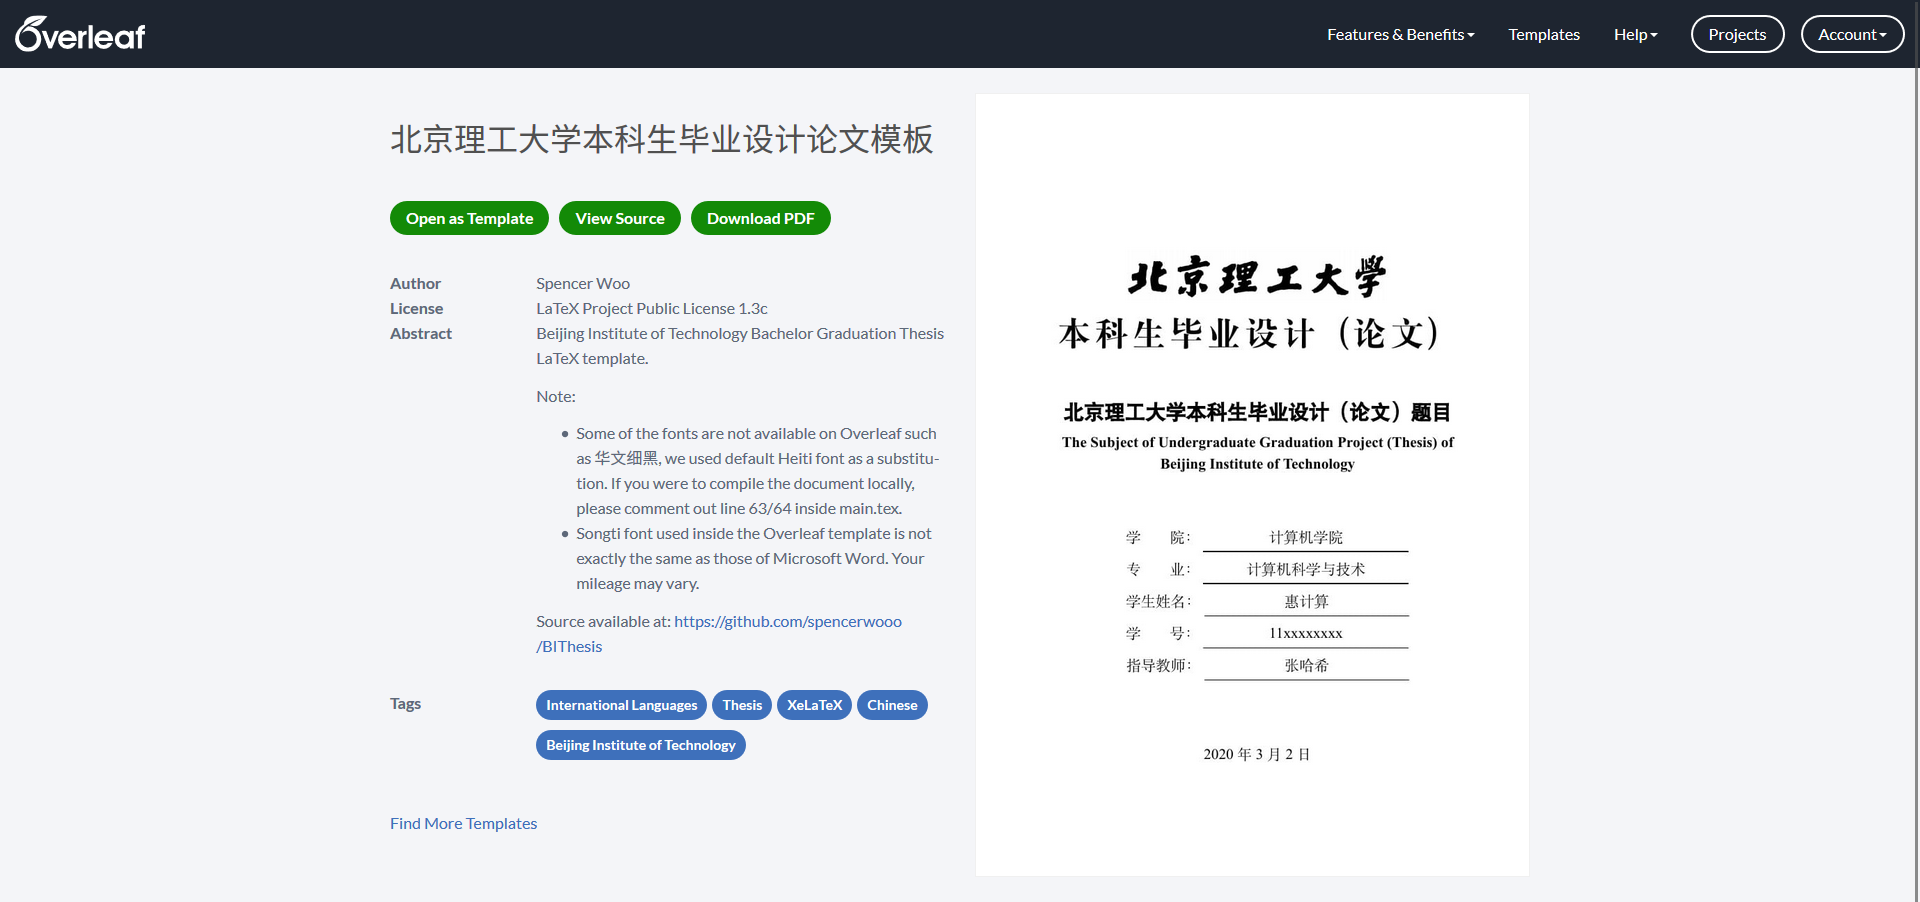
\includegraphics[width=\textwidth]{images/overleaf_grad_thesis.png}
  \caption{Overleaf 在线版本的毕业论文模板}
  \label{overleaf-grad-thesis}
\end{figure}

Overleaf 版本的毕业论文模板中由于没有微软版权字体“华文细黑”,导致封面的毕业论文中文大标题无法用 Word 模板中规定的字体渲染,使得最终呈现样式与要求有些出入,如果希望保证 {\LaTeX} 模板输出和学校模板一致,那么还是推荐在本地进行撰写和编译。

\subsection{熟悉项目}

\dirtree{%
  .1 /.
  .2 README.md.
  .2 main.tex.
  .2 main.pdf.
  .2 chapters.
  .3 0\_abstract.tex.
  .3 1\_chapter1.tex.
  .2 images.
  .3 bit\_logo.png.
  .3 header.png.
  .2 misc.
  .3 0\_cover.tex.
  .3 1\_originality.tex.
  .3 1\_originality.pdf.
  .3 2\_toc.tex.
  .3 3\_conclusion.tex.
  .3 4\_reference.tex.
  .3 5\_appendix.tex.
  .3 6\_acknowledgements.tex.
  .3 ref.bib.
}

本项目由一个主文件和与之并存的几个辅助文件夹中的文件构成:

\begin{itemize}
  \item[\color{RubineRed}\textbf{\texttt{main.tex}}] 毕业论文模板的主文件
  \item[\color{RubineRed}\textbf{\texttt{./chapters}}] 文件夹:包含有整个毕业论文的“摘要”和正文的全部“章节”
        \begin{itemize}
          \item[\color{RoyalBlue}\texttt{0\_abstract.tex}] 毕业论文的“摘要”(中文摘要与英文摘要)
          \item[\color{RoyalBlue}\texttt{1\_chapter1.tex}] 毕业论文正文“第一章”(示例章节)
          \item[\color{RoyalBlue}\texttt{...}] (你可以继续添加第二章 \texttt{2\_chapter2.tex}、第三章 \texttt{3\_chapter3.tex}……,并在主文件 \texttt{main.tex} 中引用(详见下文)
        \end{itemize}
  \item[\color{RubineRed}\textbf{\texttt{./misc}}] 文件夹:包含有毕业论文模板中的封面、后置章节与参考文献
        \begin{itemize}
          \item[\color{RoyalBlue}\textbf{\texttt{0\_cover.tex}}] 毕业论文的“封面”,一般情况无需更改
          \item[\color{RoyalBlue}\textbf{\texttt{1\_originality.tex}}] 毕业论文的“原创性声明”,一般情况无需更改(签字和日期后期手动添加)
          \item[\color{RoyalBlue}\textbf{\texttt{1\_originality.pdf}}] 毕业论文的“原创性声明”,是由原 Word 模板导出的一页 PDF 文档,插入到毕业论文中的(如果上一行中的 tex 版本格式无法满足你的需要,可以用 Word 将这一单页导出为 PDF 插入。详见源 LaTeX 代码)
          \item[\color{RoyalBlue}\textbf{\texttt{2\_toc.tex}}] 毕业论文的“目录”,一般情况无需更改(由 {\LaTeX} 自动生成)
          \item[\color{RoyalBlue}\textbf{\texttt{3\_conclusion.tex}}] 毕业论文的“结论”,按照一般章节文件对待
          \item[\color{RoyalBlue}\textbf{\texttt{4\_reference.tex}}] 毕业论文的“参考文献”,一般情况无需更改(由 {\LaTeX} 根据你文档中的 \verb|\cite{}| 自动生成)
          \item[\color{RoyalBlue}\textbf{\texttt{5\_appendix.tex}}] 毕业论文的“附录”,按照一般章节文件对待
          \item[\color{RoyalBlue}\textbf{\texttt{6\_acknow...ments.tex}}] 毕业论文的“致谢”,按照一般章节文件对待
          \item[\color{RoyalBlue}\textbf{\texttt{ref.bib}}] 参考文献 \hologo{BibTeX} 数据库
        \end{itemize}
\end{itemize}

主文件与其余文件之间的引用关系大致如下图 \ref{grad_thesis_main_submodule} 所示:

\begin{figure}[H]
  \center
  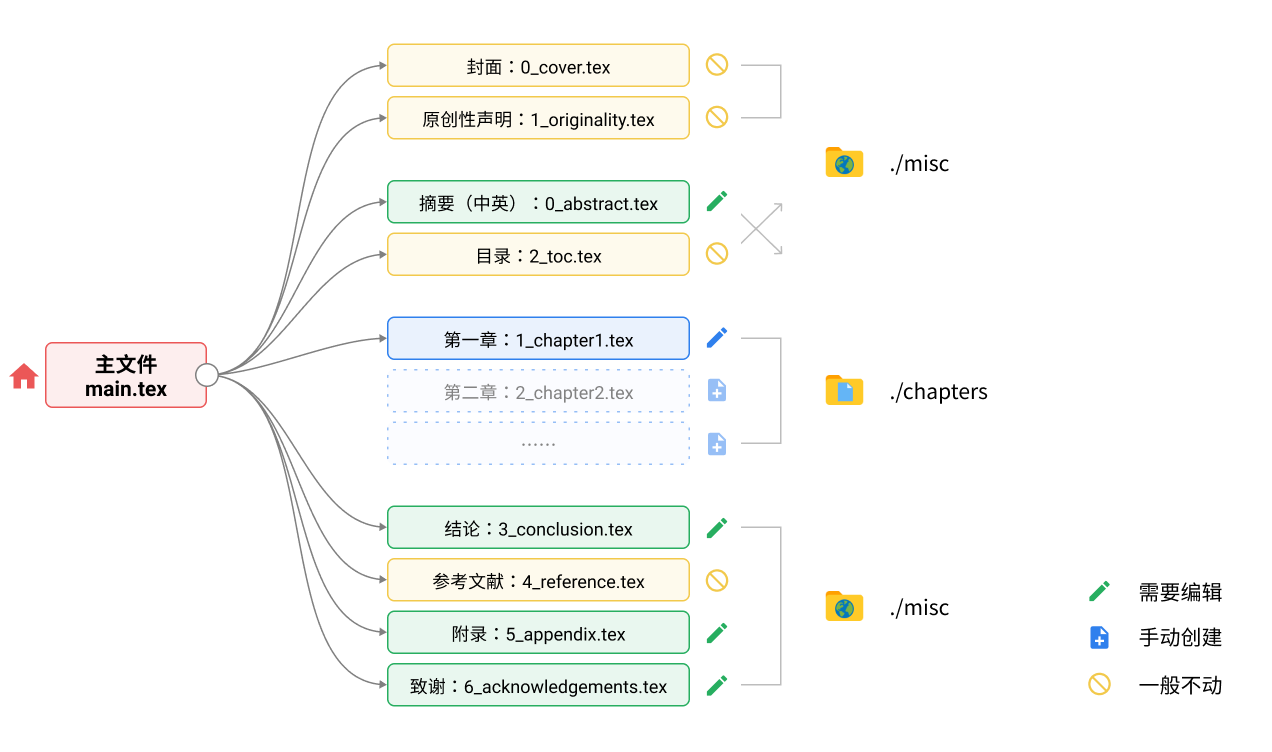
\includegraphics[width=\textwidth]{images/grad_thesis.png}
  \caption{毕业论文模板主模块与各个分支之间的关系}
  \label{grad_thesis_main_submodule}
\end{figure}

\subsection{你的内容从哪里开始?}

熟悉项目之后,你应该发现,我们毕业设计论文共分为如下的几个模块:封面、原创性声明、中英文摘要、目录、正文(多个章节)、结论、参考文献、附录与致谢。我们的整个毕业设计论文 {\LaTeX} 项目将每个模块单独提取出来,成为单独的 {\LaTeX} 文件,使用 \texttt{main.tex} 主文件统一引用,方便各位进行分模块的修改。你需要重点关注的地方有如下几个。

\subsubsection{开始}

首先,你需要定义毕业设计论文的“中文标题”和“英文标题”,这两个“变量”将影响模板封面的渲染,以及后续摘要中出现的标题的渲染。

中英文标题的定义位于 \texttt{main.tex} 的 \href{https://github.com/spencerwooo/BIThesis/blob/master/graduation-thesis/main.tex#L65-L67}{第 65 至第 67 行}:

\begin{itemize}
  \item 你可以通过控制 \texttt{\textbackslash thesisTitle} 这一变量来控制整个论文的“中文标题”
  \item 你可以通过控制 \texttt{\textbackslash thesisTitleEN} 这一变量来控制整个项目的“英文标题”
\end{itemize}

接下来,你需要定义你的个人信息,这些信息将被渲染在毕业设计论文的封面。个人信息包括你所在学院,你的专业、学号、姓名和指导教师。

个人信息的定义位于 \texttt{main.tex} 的 \href{https://github.com/spencerwooo/BIThesis/blob/master/graduation-thesis/main.tex#L69-L74}{第 69 行至第 74 行}:

\begin{itemize}
  \item \texttt{\textbackslash deptName}:你所在学院
  \item \texttt{\textbackslash majorName}:你所就读的专业
  \item \texttt{\textbackslash yourName}:你的姓名
  \item \texttt{\textbackslash yourStudentID}:你的学号
  \item \texttt{\textbackslash mentorName}:你的指导教师
\end{itemize}

\subsubsection{中英摘要}

接下来,你需要撰写论文的摘要。模板中英文摘要位于\\ \texttt{chapters/0\_abstract.tex}:

\begin{itemize}
  \item 中文摘要位于 \texttt{0\_abstract.tex} 的 \href{https://github.com/spencerwooo/BIThesis/blob/master/graduation-thesis/chapters/0_abstract.tex#L41-L48}{第 41 行至第 48 行}。其中 \href{https://github.com/spencerwooo/BIThesis/blob/master/graduation-thesis/chapters/0_abstract.tex#L48}{第 48 行} 定义摘要的中文关键词
  \item 英文摘要位于 \texttt{0\_abstract.tex} 的 \href{https://github.com/spencerwooo/BIThesis/blob/master/graduation-thesis/chapters/0_abstract.tex#L71-L76}{第 71 行至第 76 行}。其中 \href{https://github.com/spencerwooo/BIThesis/blob/master/graduation-thesis/chapters/0_abstract.tex#L76}{第 76 行} 定义摘要的英文关键词
\end{itemize}

\subsubsection{正文}

正文是一篇论文中最为重要的部分,是一篇论文的核心。正文部分可以分为多个章节,模板中仅创建了第一章节的示范性文件:\texttt{chapters/1\_chapter1.tex},你可以将它作为正文章节的“模板”,继续在 \texttt{./chapters} 目录下自行创建第二章节 \texttt{2\_chapter2.tex}、第三章节 \texttt{3\_chapter3.tex} 等等,并需要在 \texttt{main.tex} 的 \href{https://github.com/spencerwooo/BIThesis/blob/master/graduation-thesis/main.tex#L199-L203}{第 199 行} 处添加对应章节文件的相对路径引用:

\begin{minted}[frame=single]{tex}
  % 第一章
  %%
% The BIThesis Template for Bachelor Graduation Thesis
%
% 北京理工大学毕业设计(论文)第一章节 —— 使用 XeLaTeX 编译
%
% Copyright 2020-2022 BITNP
%
% This work may be distributed and/or modified under the
% conditions of the LaTeX Project Public License, either version 1.3
% of this license or (at your option) any later version.
% The latest version of this license is in
%   http://www.latex-project.org/lppl.txt
% and version 1.3 or later is part of all distributions of LaTeX
% version 2005/12/01 or later.
%
% This work has the LPPL maintenance status `maintained'.
%
% The Current Maintainer of this work is Feng Kaiyu.
%
% 第一章节

\chapter{一级题目}

\section{二级题目}
% 这里插入一个参考文献,仅作参考

\subsection{三级题目}

正文……\cite{yuFeiJiZongTiDuoXueKeSheJiYouHuaDeXianZhuangYuFaZhanFangXiang2008}……\cite{Hajela2012Application}

\textcolor{blue}{正文部分:宋体、小四;正文行距:22磅;间距段前段后均为0行。阅后删除此段。}

\textcolor{blue}{图、表居中,图注标在图下方,表头标在表上方,宋体、五号、居中,1.25倍行距,间距段前段后均为0行,图表与上下文之间各空一行。阅后删除此段。}

\textcolor{blue}{\underline{\underline{图-示例:(阅后删除此段)}}}


\begin{figure}[htbp]
  \centering
  
\includegraphics[]{images/bit_logo.png}
  \caption{标题序号}\label{标题序号} % label 用来在文中索引
\end{figure}

\textcolor{blue}{\underline{\underline{表-示例:(阅后删除此段)}}}
% 三线表
\begin{table}[htbp]
  \linespread{1.5}
  \zihao{5}
  \centering
  \caption{统计表}\label{统计表}
  \begin{tabular}{*{5}{>{\centering\arraybackslash}p{2cm}}} \toprule
    项目    & 产量    & 销量    & 产值   & 比重    \\ \hline
    手机    & 1000  & 10000 & 500  & 50\%  \\
    计算机   & 5500  & 5000  & 220  & 22\%  \\
    笔记本电脑 & 1100  & 1000  & 280  & 28\%  \\
    合计    & 17600 & 16000 & 1000 & 100\% \\ \bottomrule
    \end{tabular}
\end{table}

\textcolor{blue}{公式标注应于该公式所在行的最右侧。对于较长的公式只可在符号处(+、-、*、/、$\leqslant$ $\geqslant$ 等)转行。在文中引用公式时,在标号前加“式”,如式(1-2)。阅后删除此
段。}

\textcolor{blue}{公式-示例:(阅后删除此段)}
% 公式上下不要空行,置于同一个段落下即可,否则上下距离会出现高度不一致的问题
\begin{equation}
    LRI=1\ ∕\ \sqrt{1+{\left(\frac{{\mu }_{R}}{{\mu }_{s}}\right)}^{2}{\left(\frac{{\delta }_{R}}{{\delta }_{s}}\right)}^{2}}
\end{equation}

\subsubsection{生僻字}

% 一个可能无法正常显示的生僻字
一个可能无法正常显示的生僻字: 彧。下文注释中,介绍了如何通过自定义字体来显示生僻字。

% 定义一个提供了生僻字的字体,注意要确保你的系统存在该字体
% \setCJKfamilyfont{custom-font}{Noto Serif CJK SC}

% 使用自己定义的字体
% 使用提供了相应字型的字体:\CJKfamily{custom-font}{彧}。


  % 在这里添加第二章、第三章……TeX 文件的引用
  %%
% The BIThesis Template for Bachelor Graduation Thesis
%
% 北京理工大学毕业设计(论文)第二章节 —— 使用 XeLaTeX 编译
%
% Copyright 2020-2021 BITNP
%
% This work may be distributed and/or modified under the
% conditions of the LaTeX Project Public License, either version 1.3
% of this license or (at your option) any later version.
% The latest version of this license is in
%   http://www.latex-project.org/lppl.txt
% and version 1.3 or later is part of all distributions of LaTeX
% version 2005/12/01 or later.
%
% This work has the LPPL maintenance status `maintained'.
%
% The Current Maintainer of this work is Feng Kaiyu.
%%

\chapter{另一个章节}

\section{代码片段}

\begin{lstlisting}[language=Python, caption={Python Code}, label={lst:pythonfile}]
import numpy as np

def incmatrix(genl1,genl2):
    m = len(genl1)
    n = len(genl2)
    M = None #to become the incidence matrix
    VT = np.zeros((n*m,1), int)  #dummy variable

    #compute the bitwise xor matrix
    M1 = bitxormatrix(genl1)
    M2 = np.triu(bitxormatrix(genl2),1)

    for i in range(m-1):
        for j in range(i+1, m):
            [r,c] = np.where(M2 == M1[i,j])
            for k in range(len(r)):
                VT[(i)*n + r[k]] = 1;
                VT[(i)*n + c[k]] = 1;
                VT[(j)*n + r[k]] = 1;
                VT[(j)*n + c[k]] = 1;

                if M is None:
                    M = np.copy(VT)
                else:
                    M = np.concatenate((M, VT), 1)

                VT = np.zeros((n*m,1), int)

    return M
\end{lstlisting}

  \chapter{Engineering Design}

Although engineering drawing still plays an important role in product design and manufacturing in many industrial sectors around the world, manual sketching for creating drawings has been gradually replaced by CAD (computer-aided design) software using computers. Beginning in the 1980s, CAD software reduced the need for draftsmen significantly, especially in small to mid-sized companies. The software’s affordability and ability to run on personal computers in the mid-1990s allowed engineers to do their own drafting and analytic work to some extent \ref{eq:1}.

\begin{equation}
x^n + y^n = z^n
\label{eq:1}
\end{equation}

\end{minted}

之后,你可以分别在每个章节独立的 \TeX 文件中撰写每一章节的内容。

\subsubsection{后续模块}

在正文之后,我们的论文还剩下:结论、参考文献、附录与致谢这四个模块。它们依次位于:

\begin{itemize}
  \item Conclusion 结论:\texttt{misc/3\_conclusion.tex}
  \item Reference 参考文献:\texttt{misc/4\_reference.tex}
  \item Appendix 附录:\texttt{misc/5\_appendix.tex}
  \item Acknowledgements 致谢:\texttt{misc/6\_acknowledgements.tex}
\end{itemize}

其中,你不需要手动编辑“参考文献”这一文件,只需要撰写“结论”、“附录”和“致谢”即可。这三个模块的撰写逻辑与前面正文章节的撰写逻辑是一致的。

\tipbox{有关具体的 {\LaTeX} 语法,请参考前文中《第二章 \ref{subsec:latex-grammar}》给出的参考链接与学习文档。接下来是模板中提供的一些示例性代码的使用方法。}

\subsection{参考文献管理}

为了保证你的毕业论文的参考文献格式标准,你需要将参考文献的 \hologo{BibTeX} 引用复制进入 \texttt{./misc/refs.bib},并在正文中用 \verb|\cite{xxx}| 的方法进行引用。

\hologo{BibTeX} 是一种表示、存储与引用参考文献的语法,谷歌学术中搜索文章直接复制得到,如图 \ref{google_scholar} 所示:

\begin{figure}[H]
  \center
  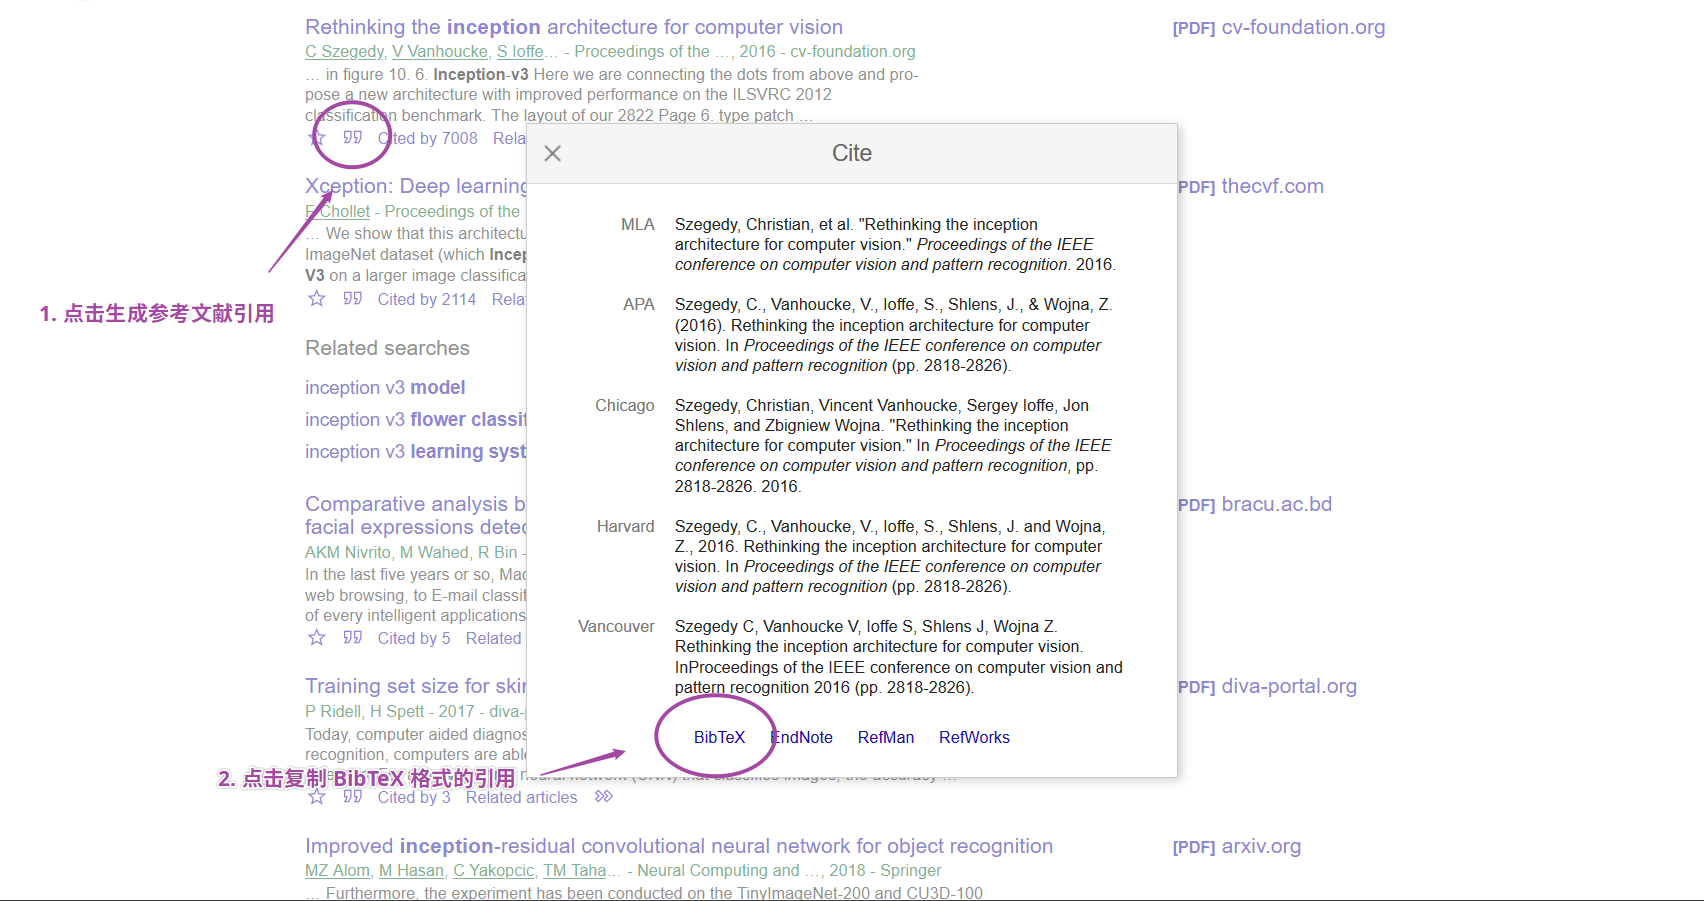
\includegraphics[width=\textwidth]{images/google_scholar.png}
  \caption{谷歌学术搜索并复制文献的 \hologo{BibTeX} 格式}
  \label{google_scholar}
\end{figure}

复制得到的参考文献 \hologo{BibTeX} 类似:

\begin{minted}[frame=single,linenos,breaklines]{tex}
  @inproceedings{szegedy2016rethinking,
    title={Rethinking the inception architecture for computer vision},
    author={Szegedy, Christian and Vanhoucke, Vincent and Ioffe, Sergey and Shlens, Jon and Wojna, Zbigniew},
    booktitle={Proceedings of the IEEE conference on computer vision and pattern recognition},
    pages={2818--2826},
    year={2016}
  }
\end{minted}

将上面的内容复制进入 \texttt{misc/ref.bib} 即可,之后你就可以直接在文章中使用这一参考文献的地方用类似下面的方法引用这一标签为 szegedy2016rethinking 的参考文献:

\begin{minted}[frame=single,linenos,breaklines]{tex}
  正文,正文正文 \cite{szegedy2016rethinking} 正文正文……
\end{minted}

另外,你也可以考虑使用 Zotero 等专业文献管理工具批量生成。参考:\href{https://sspai.com/post/56724}{文献管理神器 Zotero 学习路径指南}。

\begin{figure}[H]
  \center
  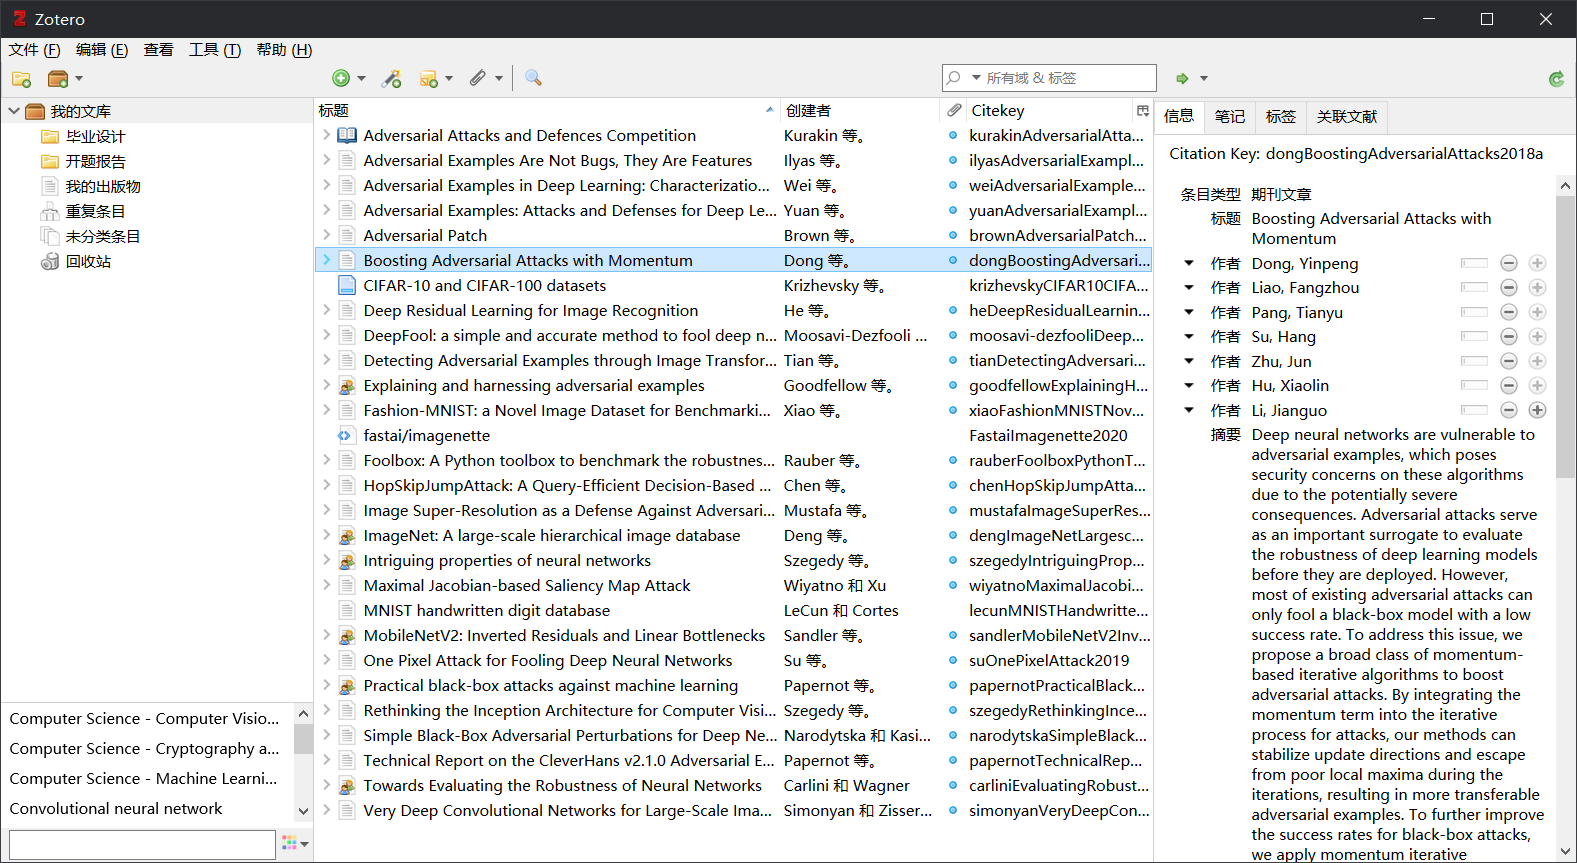
\includegraphics[width=\textwidth]{images/zotero.png}
  \caption{专业文献管理工具 Zotero}
\end{figure}

\subsection{图片素材}

整个模板的图片素材都整理在图片文件夹中:\texttt{./images}。你可以将论文中使用到的图片统一放在这一目录下进行管理,在论文中使用“相对路径”进行引用。你可以用类似下面的语法引用图片:

\begin{minted}[frame=single,linenos,breaklines]{tex}
  \begin{figure}[htbp]
    \vspace{13pt} % 调整图片与上文的垂直距离
    \centering
    
\includegraphics[width=0.8\textwidth]{images/bit_logo.png}
    \caption{标题序号}
    \label{标题序号} % label 用来在文中索引
  \end{figure}
\end{minted}

可以看到:

\begin{itemize}
  \item 我们首先将图片放置在了一个 \verb|\begin{figure} ... \end{figure}| 的环境中,其中 \texttt{[htbp]} 是用于定位图片。
  \item 之后,在环境中,我们首先使用 \verb|\centering| 保证图片水平居中
  \item 之后用 \verb|\includegraphics[图片大小]{图片路径}| 的格式引用了图片本身(图片大小的语法 \verb|width=0.8\textwidth| 表示图片宽度是整个页宽的 0.8 倍)
  \item 最后我们定义了图片的说明文字 \verb|\caption{图片说明}| 和图片的标签编号 \verb|\label{图片编号}|,前者显示在图片下方起到说明注释的作用,后者让我们可以用 \verb|\ref{图片编号}| 的语法来在正文中引用图片
\end{itemize}

请注意,为了保证图片引用的格式和 Word 模板完全一致,我们手动设置了 \verb|\vspace{13pt}| 的垂直空白,你引用新图片时,也需要添加这一垂直空白。

在第一章节 \texttt{chapters/1\_chapter1.tex} 中的 \href{https://github.com/spencerwooo/BIThesis/blob/master/graduation-thesis/chapters/1_chapter1.tex#L38-L43}{第 38 行至第 43 行} 是一个示范。

\subsection{表格插入}

表格一直是 {\LaTeX} 排版系统非常强大又非常不好实现的一个模块,如果你希望方便的插入表格,可以统一使用 \href{https://www.tablesgenerator.com/}{LaTeX Tables Generator} 进行生成,再粘贴进入模板之中。

在第一章节 \texttt{chapters/1\_chapter1.tex} 中的 \href{https://github.com/spencerwooo/BIThesis/blob/master/graduation-thesis/chapters/1_chapter1.tex#L47-L60}{第 47 行至第 60 行} 是一个示范。

\subsection{公式插入}

{\LaTeX} 的行内数学符号和公式等,使用 \verb|\( ... \)| 的语法进行定义。比如类似如下的正文:

\begin{minted}[frame=single,linenos,breaklines]{tex}
  The well known Pythagorean theorem \(x^2 + y^2 = z^2\) was
  proved to be invalid for other exponents.
  Meaning the next equation has no integer solutions:

  \[ x^n + y^n = z^n \]
\end{minted}

即可非常简单的渲染如下的公式效果:

The well known Pythagorean theorem \(x^2 + y^2 = z^2\) was proved to be invalid for other exponents. Meaning the next equation has no integer solutions:

\[ x^n + y^n = z^n \]

另外,行内数学环境也可以用 \verb|$ ... $| 的语法进行定义:

\begin{minted}[frame=single,linenos,breaklines]{tex}
  In physics, the mass-energy equivalence is stated
  by the equation $E=mc^2$, discovered in 1905 by Albert Einstein.
\end{minted}

In physics, the mass-energy equivalence is stated
by the equation $E=mc^2$, discovered in 1905 by Albert Einstein.

复杂的独立模块数学公式可以用如下的语法进行定义:

\begin{minted}[frame=single,linenos,breaklines]{tex}
  \begin{equation}
    LRI=1\ ∕\ \sqrt{1+{\left(\frac{{\mu }_{R}}{{\mu }_{s}}\right)}^{2}{\left(\frac{{\delta }_{R}}{{\delta }_{s}}\right)}^{2}}
  \end{equation}
\end{minted}

\begin{equation}
  LRI=1\ ∕\ \sqrt{1+{\left(\frac{{\mu }_{R}}{{\mu }_{s}}\right)}^{2}{\left(\frac{{\delta }_{R}}{{\delta }_{s}}\right)}^{2}}
\end{equation}

为了保证与 Word 模板中的数学公式要求一致,我们的 {\LaTeX} 模板中的公式默认会进行相应的编号(比如上面的例子)。在第一章节 \texttt{chapters/1\_chapter1.tex} 中的 \href{https://github.com/spencerwooo/BIThesis/blob/master/graduation-thesis/chapters/1_chapter1.tex#L67-L69}{第 67 行至第 69 行} 是一个示范。

\subsection{其他}

以下模块的使用可能需要你手动在 \texttt{main.tex} 的开头用 \verb|\usepackage{ ... }| 的方法引入其他 {\LaTeX} 宏包。

\subsubsection{代码高亮}

你可以使用 \texttt{minted} 宏包来进行代码块的渲染。比如:

\begin{itemize}
  \item 在文档开题引入宏包:
        \begin{minted}[frame=single]{tex}
    \usepackage{minted}
  \end{minted}
  \item 渲染代码块:
        \begin{minted}[frame=single]{tex}
    \begin{minted}{python}
      import numpy as np

      def incmatrix(genl1,genl2):
        m = len(genl1)
        n = len(genl2)
        M = None #to become the incidence matrix
        VT = np.zeros((n*m,1), int)  #dummy variable

        #compute the bitwise xor matrix
        M1 = bitxormatrix(genl1)
        M2 = np.triu(bitxormatrix(genl2),1)
    \end{mintd}
  \end{minted}
\end{itemize}

你就会得到类似下面的渲染效果:

\begin{minted}[frame=single]{python}
import numpy as np

def incmatrix(genl1,genl2):
  m = len(genl1)
  n = len(genl2)
  M = None #to become the incidence matrix
  VT = np.zeros((n*m,1), int)  #dummy variable

  #compute the bitwise xor matrix
  M1 = bitxormatrix(genl1)
  M2 = np.triu(bitxormatrix(genl2),1)
\end{minted}

有关 \texttt{minted} 的更多使用方法,请阅读:\href{https://www.overleaf.com/learn/latex/Code_Highlighting_with_minted}{Code Highlighting with minted。}

如果你在使用 \texttt{minted} 的过程中遇到了任何问题,请阅读:《第 \ref{sec:troubleshooting} 章:疑难杂症 Troubleshooting》。

\subsubsection{算法模块}

你可以使用 algorithm2e 宏包来渲染一个“伪代码算法”模块。比如:

\begin{itemize}
  \item 在文档开头引入宏包:
        \begin{minted}[frame=single]{tex}
    \usepackage[ruled,vlined]{algorithm2e}
  \end{minted}
  \item 渲染伪代码模块:
        \begin{minted}[frame=single]{tex}
    \begin{algorithm}[H]
    \SetAlgoLined
    \KwResult{Write here the result }
      initialization\;
      \While{While condition}{
      instructions\;
      \eIf{condition}{
        instructions1\;
        instructions2\;
        }{
        instructions3\;
        }
      }
    \caption{How to write algorithms}
    \end{algorithm}
  \end{minted}
\end{itemize}

这样,你就会得到类似如下的渲染效果:

\begin{algorithm}[H]
  \SetAlgoLined
  \KwResult{Write here the result }
  initialization\;
  \While{While condition}{
    instructions\;
    \eIf{condition}{
      instructions1\;
      instructions2\;
    }{
      instructions3\;
    }
  }
  \caption{How to write algorithms}
\end{algorithm}

有关更多伪代码算法模块的使用,请阅读:\href{https://www.overleaf.com/learn/latex/algorithms}{Algorithms}。
